\documentclass[10pt, a4paper]{article}
\usepackage{cmap}
\usepackage[T2A]{fontenc}
\usepackage[utf8]{inputenc}
\usepackage[english, russian]{babel}
\usepackage[dvipsnames,table,xcdraw]{xcolor}
\usepackage{
	amsmath,
	amssymb,
	scrextend,
	enumitem,
	pscyr,
	multicol,
	cmap,
	titling,
	indentfirst,
	cancel,
	wrapfig,
	gensymb,
	tikz,
	graphicx,
	fancyhdr,
	mathrsfs,
	graphbox,
	indentfirst
}
%Параметры страницы
\usepackage[left=15mm,right=15mm,
top=2cm,bottom=2cm]{geometry}
\pagestyle{fancy}
%Путь к картинкам
\graphicspath{{pic/}}
\DeclareGraphicsExtensions{.pdf,.png,.jpg}
%Числа в списке второго уровня по умолчанию
\renewcommand{\labelenumii}{\arabic{enumii})}
%Новые команды
\newcommand{\answer}[1]{\textcolor[rgb]{0.8,0.8,0.8}{\fbox{\scriptsize=#1}}}

%Русские символы в списке
\AddEnumerateCounter{\asbuk}{\russian@alph}{щ}

%Сеттеры
\setlength{\parindent}{5ex}
\setlength{\parskip}{1em}

\begin{document}
%Сеттеры

\setlength{\abovedisplayskip}{2pt}
		
\lhead{Функции}
\rhead{Школа <<Симметрия>>}

\begin{center}
	\Large \textbf{Преобразования графиков функций} 
\end{center}
\begin{enumerate}
	% #1
	\item \textbf{Смещение графика функции по горизонтали [\boldmath$y=f(x+c)$]}\\[1em]
	Если к аргументу функции $y=f(x)$ прибавить число $c$, то график функции $y=f(x)$ сместится по горизонтали.
	\begin{enumerate}[label=\asbuk*)]
		\begin{minipage}[t]{0.4\textwidth}
			\item \textbf{Если \boldmath$c>0$}, то график $f(x)$ сместится \textbf{влево} на $c$:
			\vspace{1em}
			\begin{center}
				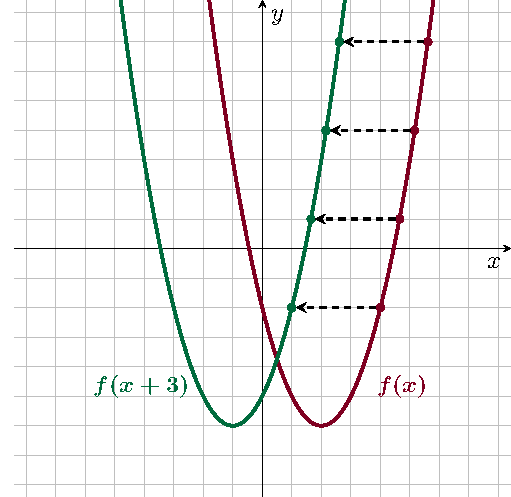
\includegraphics[align=t, width=0.6\textwidth]{../graphs/graph_2/graph_2}
			\end{center}
		\end{minipage}
		\hspace{0.1\textwidth}
		\begin{minipage}[t]{0.4\textwidth}
			\item \textbf{Если \boldmath$c<0$}, то график $f(x)$ сместится \textbf{вправо} на $|c|$:
			\vspace{1em}
			\begin{center}
				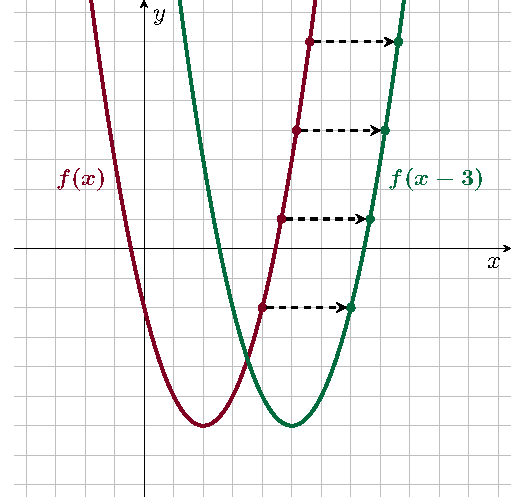
\includegraphics[align=t, width=0.6\textwidth]{../graphs/graph_3/graph_3}
			\end{center}
		\end{minipage}
	\end{enumerate}
	% #2
	\item \textbf{Смещение графика функции по вертикали [\boldmath$y=f(x)+c$]}\\[1em]
	Если к функции $y=f(x)$ прибавить число $c$, то график функции $y=f(x)$ сместится по вертикали.\\
	\begin{enumerate}[label=\asbuk*)]
		\begin{minipage}[t]{0.4\textwidth}
			\item Если $c>0$, то график $f(x)$ сместится \textbf{вверх} на $c$:
			\vspace{1em}
			\begin{center}
				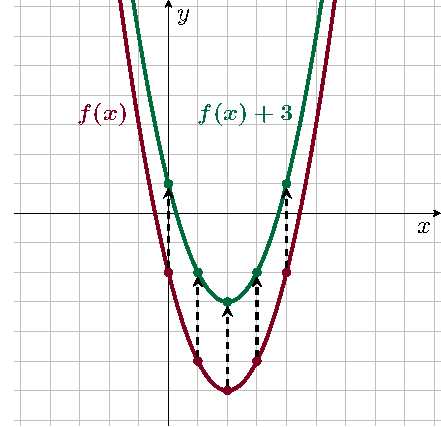
\includegraphics[align=t, width=0.6\textwidth]{../graphs/graph_4/graph_4}
			\end{center}
		\end{minipage}
		\hspace{0.1\textwidth}
		\begin{minipage}[t]{0.4\textwidth}
			\item Если $c<0$, то график $f(x)$ сместится \textbf{вниз} на $|c|$:
			\vspace{1em}
			\begin{center}
				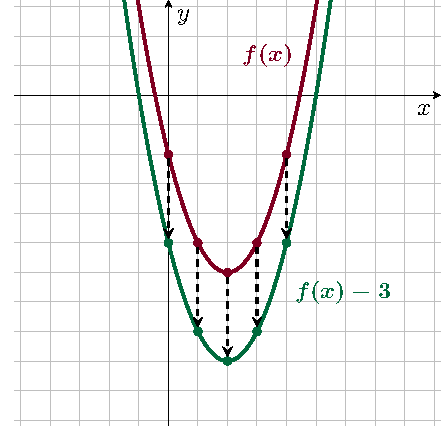
\includegraphics[align=t, width=0.6\textwidth]{../graphs/graph_5/graph_5}
		\end{center}
		\end{minipage}
	\end{enumerate}
	% #3
	\item \textbf{Растяжение или сжатие графика по вертикали [\boldmath$y=c\cdot f(x)$]}\\[1em]
	Если всю функцию $y=f(x)$ умножить на число $c$, то график функции $y=f(x)$ может растянуться, сжаться или отразиться относительно оси $X$ в зависимости от значения $c$. Рассмотрим каждый случай отдельно.
	
	Сразу обратим внимание, что точки, которые называют нули функции (точки, у которых $y=0$), в любом случае не меняют своего положения.
	\begin{enumerate}[label=\asbuk*), itemsep=1em]
		\item 
		\begin{minipage}[t]{0.65\textwidth}
			\textbf{Если \boldmath$ c>1$}, то график функции \textbf{растянется от оси $\boldsymbol X$}.\smallskip
			
			Игрековые координаты всех точек графика изменятся в $c$ раз. Это означает, что точки графика, у которых $y>0$, сместятся в $c$ раз вверх, а точки с отрицательными значениями по игреку сместятся в $c$ раз вниз.
		\end{minipage}
		\begin{minipage}[t]{0.25\textwidth}
			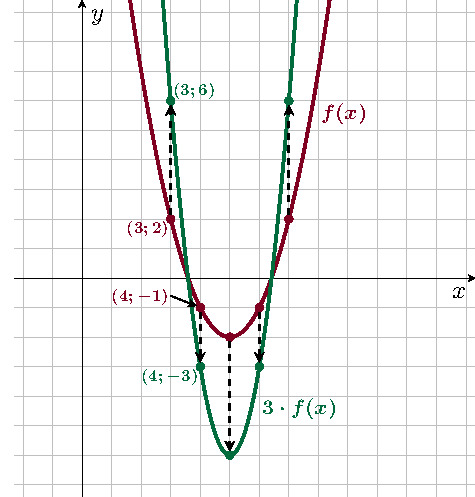
\includegraphics[align=t, width=\textwidth]{../graphs/graph_6/graph_6}
		\end{minipage}
		\item
		\begin{minipage}[t]{0.65\textwidth}
			\textbf{Если \boldmath$0<c<1$}, то график функции \textbf{сожмется к оси $\boldsymbol X$}.\smallskip
			
			В этом случае точки графика, у которых $y>0$, сместятся в $\frac{1}{c}$ раза вниз, а те, у которых $y<0$, сместятся в $\frac{1}{c}$ раза вверх.
		\end{minipage}
		\begin{minipage}[t]{0.25\textwidth}
			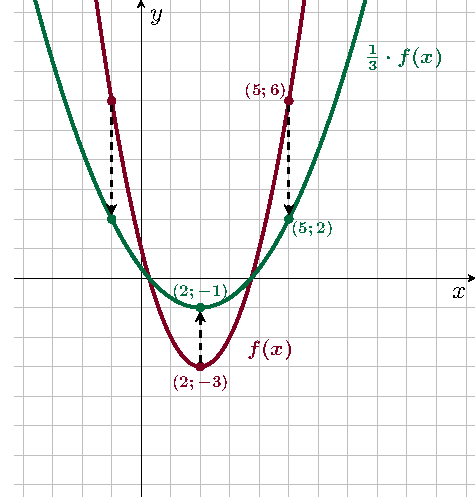
\includegraphics[align=t, width=\textwidth]{../graphs/graph_7/graph_7}
		\end{minipage}
		\item
		\begin{minipage}[t]{0.65\textwidth}
			\textbf{Если \boldmath$c=0$}, то уравнение функции \textbf{превратится в уравнение \boldmath$y=0$}.\smallskip
			
			Очевидно, что при умножении всего выражения $f(x)$ на $0$ в результате получим $0$ и уравнение функции будет $y=0\cdot f(x)=0$, то есть $y=0$. Вспомним, что график функции вида $y=a$, где $a$ — число, это прямая линия, параллельная оси $X$ и пересекающая ось $Y$ в значении $a$. В нашем случае получим прямую, проходящую по оси $X$.
		\end{minipage}
		\begin{minipage}[t]{0.25\textwidth}
			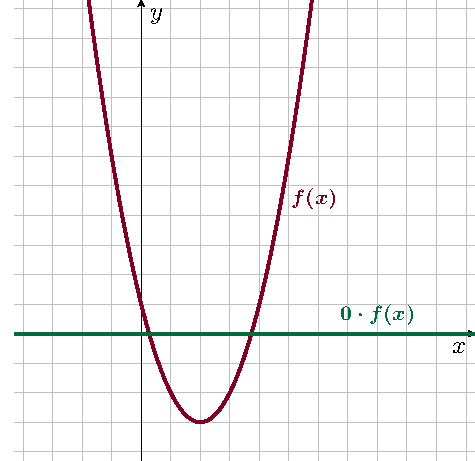
\includegraphics[align=t, width=\textwidth]{../graphs/graph_10/graph_10}
		\end{minipage}
		\item
		\begin{minipage}[t]{0.65\textwidth}
			\textbf{Если \boldmath$c=-1$}, то график функции \textbf{отразится относительно оси $\boldsymbol X$}.\smallskip
			
			В этом случае игрековые координаты всех точек графика функции изменятся на противоположные.
		\end{minipage}
		\begin{minipage}[t]{0.25\textwidth}
			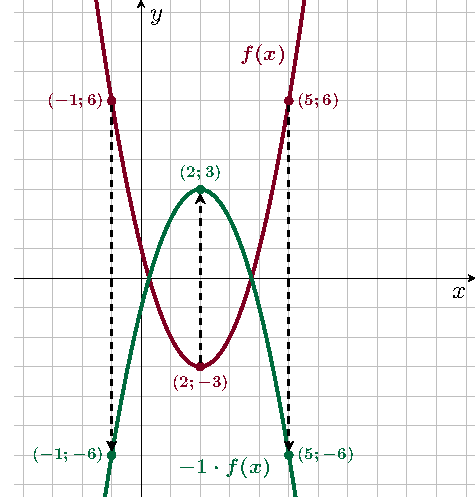
\includegraphics[align=t, width=\textwidth]{../graphs/graph_8/graph_8}
		\end{minipage}
		\item
		\begin{minipage}[t]{0.65\textwidth}
			\textbf{Если \boldmath$-1<c<0$}, то график функции \textbf{отразится относительно оси $\boldsymbol X$} и \textbf{сожмется к оси $\boldsymbol X$} в $\frac{1}{|c|}$ раз.\smallskip
			
			Такое преобразование удобно делать в два приема: сначала отражаем график относительно оси $X$ график, а потом сжимаем к оси $X$.
		\end{minipage}
		\begin{minipage}[t]{0.25\textwidth}
			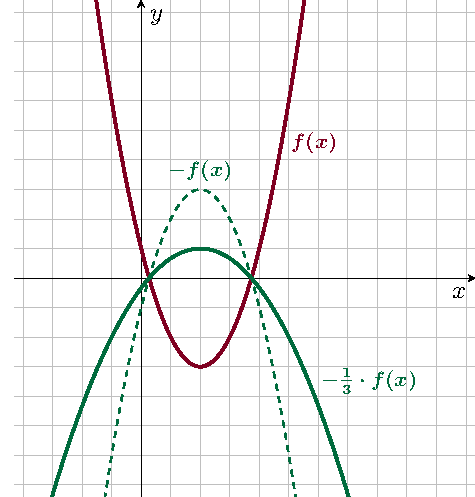
\includegraphics[align=t, width=\textwidth]{../graphs/graph_9/graph_9}
		\end{minipage}
		\item
		\begin{minipage}[t]{0.65\textwidth}
			\textbf{Если \boldmath$c < -1$}, то график функции \textbf{отразится относительно оси $\boldsymbol X$} и \textbf{растянется от оси $\boldsymbol X$} в ${|c|}$ раз.\smallskip
			
			Это преобразование делаем также в два приема: сначала отражаем график относительно оси $X$ график, а потом растягиваем от оси $X$.
		\end{minipage}
		\begin{minipage}[t]{0.25\textwidth}
			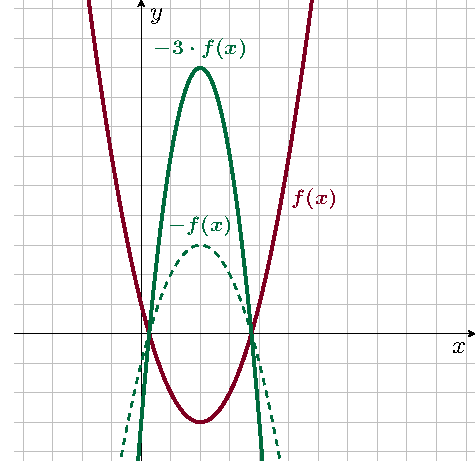
\includegraphics[align=t, width=\textwidth]{../graphs/graph_11/graph_11}
		\end{minipage}
	\end{enumerate}
	\newpage
	% #4
	\item \textbf{Растяжение от или сжатие к оси $\boldsymbol Y$ [\boldmath$y=f(c\cdot x)$]}\\[1em]
	Если аргумент функции $y=f(x)$ умножить на число $c$, то график функции $y=f(x)$ может растянуться, сжаться или отразиться относительно оси $Y$ в зависимости от значения $c$. Также как и в предыдущем пункте рассмотрим каждый случай отдельно.\smallskip
	
	В этом случае стоит отметить, что точка пересечения графика с осю $Y$ не меняет своего положения.
	\begin{enumerate}[label=\asbuk*), itemsep=1em]
		\item 
		\begin{minipage}[t]{0.65\textwidth}
			\textbf{Если \boldmath$c>1$}, то график функции \textbf{сожмется к оси $\boldsymbol Y$}.\smallskip
			
			Иксовые координаты всех точек графика изменятся в $c$ раз. То есть точки графика, у которых $x>0$, сместятся в $c$ раз влево, а точки, у которых $x<0$, сместятся в $c$ раз вправо.
		\end{minipage}
		\begin{minipage}[t]{0.25\textwidth}
			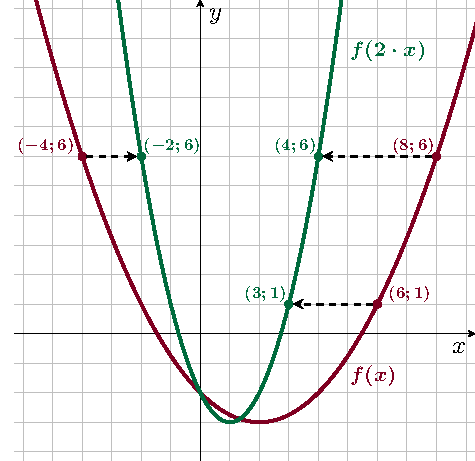
\includegraphics[align=t, width=\textwidth]{../graphs/graph_12/graph_12}
		\end{minipage}
		\item 
		\begin{minipage}[t]{0.65\textwidth}
			\textbf{Если \boldmath$0<c<1$}, то график функции \textbf{растянется от оси $\boldsymbol Y$}.\smallskip
			
			Точки графика, у которых $x>0$, сместятся в $\frac{1}{c}$ раза влево, а точки, у которых $x<0$, сместятся в $\frac{1}{c}$ раз вправо.
		\end{minipage}
		\begin{minipage}[t]{0.25\textwidth}
			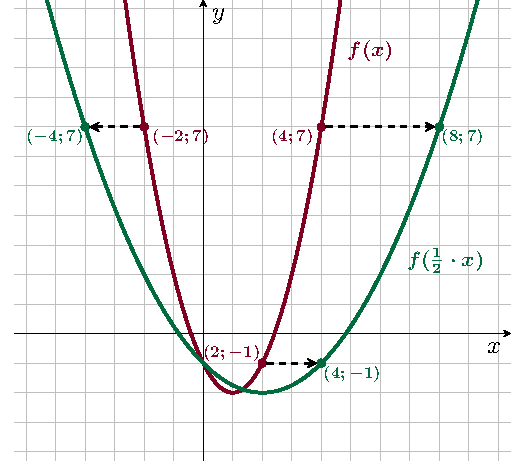
\includegraphics[align=t, width=\textwidth]{../graphs/graph_13/graph_13}
		\end{minipage}
		\item 
		\begin{minipage}[t]{0.65\textwidth}
			\textbf{Если \boldmath$c=0$}, то график функции \textbf{превратится в уравнение \boldmath$y=a$}, где $a$ — точка, в которой график пересекает ось $Y$.\smallskip
			
			Рассмотрим пример, представленный на рисунке справа.
			График функции $f(x)$ задан выражением $f(x)=x^2-2x-1$. Умножим аргумент функции на $0$:
			$$f(0\cdot x) = (0\cdot x)^2 - 2 (0\cdot x) - 1 = 0^2 - 2\cdot 0 - 1 = 0 - 0 - 1 = -1$$
			То есть $f(0 \cdot x) = -1$. Графиком такой функции является прямая линия, параллельная оси $X$, пересекающая ось $Y$ в точке $-1$.
		\end{minipage}
		\begin{minipage}[t]{0.25\textwidth}
			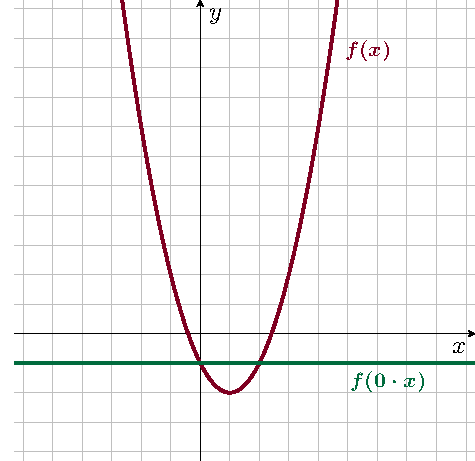
\includegraphics[align=t, width=\textwidth]{../graphs/graph_14/graph_14}
		\end{minipage}
		\item 
		\begin{minipage}[t]{0.65\textwidth}
			\textbf{Если \boldmath$c=-1$}, то график функции \textbf{отразится относительно оси $\boldsymbol Y$}.\smallskip
			
			В этом случае иксовые координаты всех точек графика функции изменятся на противоположные.
		\end{minipage}
		\begin{minipage}[t]{0.25\textwidth}
			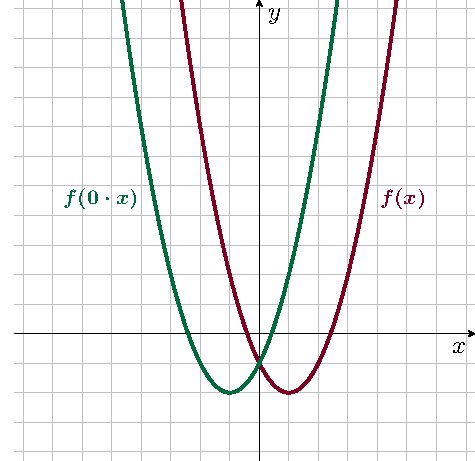
\includegraphics[align=t, width=\textwidth]{../graphs/graph_15/graph_15}
		\end{minipage}
		\item 
		\begin{minipage}[t]{0.65\textwidth}
			\textbf{Если \boldmath$-1<c<0$}, то график функции \textbf{отразится относительно оси $\boldsymbol Y$} и \textbf{растянется от оси $\boldsymbol Y$} в $\frac{1}{|c|}$ раз.\smallskip
			
			Это преобразование делаем также в два приема: сначала отражаем график относительно оси $Y$, а потом растягиваем от оси $Y$.
		\end{minipage}
		\begin{minipage}[t]{0.25\textwidth}
			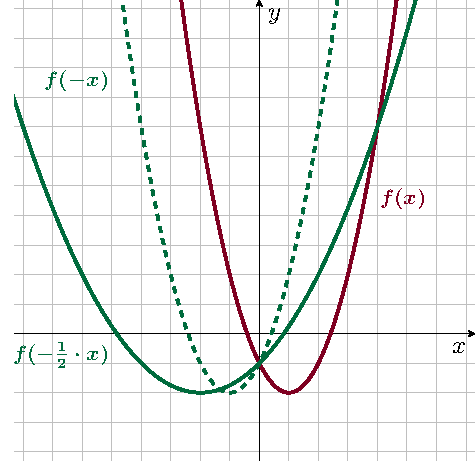
\includegraphics[align=t, width=\textwidth]{../graphs/graph_16/graph_16}
		\end{minipage}
		\item 
		\begin{minipage}[t]{0.65\textwidth}
			\textbf{Если \boldmath$c< -1$}, то график функции \textbf{отразится относительно оси $\boldsymbol Y$} и \textbf{сожмется к оси $\boldsymbol Y$} в $|c|$ раз.\smallskip
			
			Это преобразование делаем снова в два приема: сначала отражаем график относительно оси $Y$, а потом сжимаем к оси $Y$.
		\end{minipage}
		\begin{minipage}[t]{0.25\textwidth}
			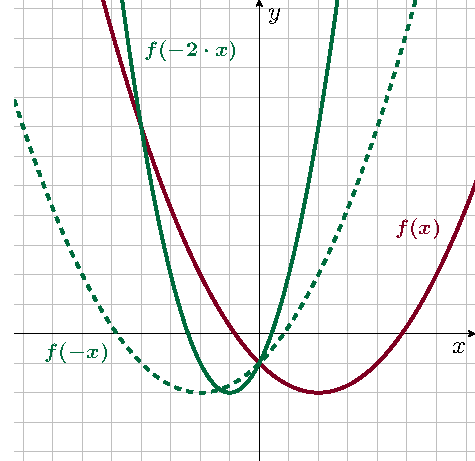
\includegraphics[align=t, width=\textwidth]{../graphs/graph_17/graph_17}
		\end{minipage}
	\end{enumerate}
	% #5
	\item \textbf{Отражение части графика относительно оси $\boldsymbol X$ [\boldmath$y=|f(x)|$]}\\[1em]
	Если всю функцию $y=f(x)$ взять по модулю, то часть графика функции $y=f(x)$, которая расположена ниже оси $X$, отразится относительно оси $X$.\smallskip
	
	\begin{minipage}[t]{0.45\textwidth}
		\begin{center}
			Исходный график $y=f(x)$\smallskip
			
			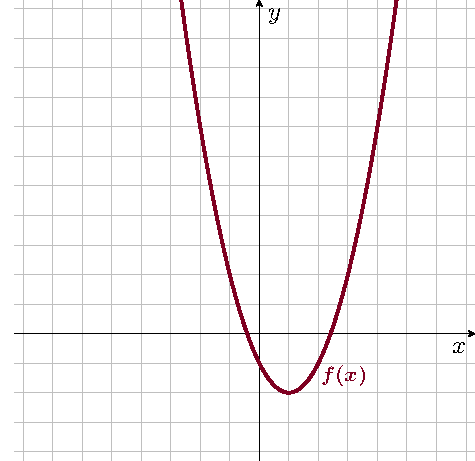
\includegraphics[align=t, width=0.5\textwidth]{../graphs/graph_18/graph_18}
		\end{center}
	\end{minipage}
	\begin{minipage}[t]{0.45\textwidth}
		\begin{center}
			График функции $y=|f(x)|$\smallskip
			
			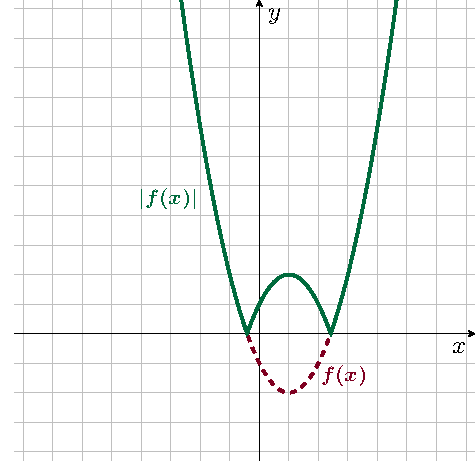
\includegraphics[align=t, width=0.5\textwidth]{../graphs/graph_18_2/graph_18_2}
		\end{center}
	\end{minipage}
	% #6
	\item \textbf{Отражение части графика относительно оси $\boldsymbol Y$ [\boldmath$y=f(|x|)$]}\\[1em]
	Если аргумент функции $y=f(x)$ взять по модулю, то часть графика функции $y=f(x)$, которая расположена левее оси $Y$, сотрется, а правая часть отразится относительно оси $Y$.\smallskip
	
	\begin{minipage}[t]{0.45\textwidth}
		\begin{center}
			Исходный график $y=f(x)$\smallskip
			
			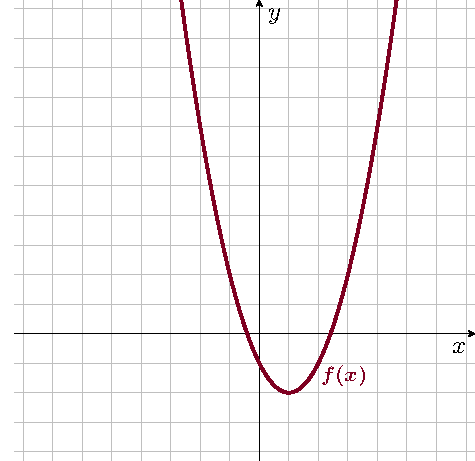
\includegraphics[align=t, width=0.5\textwidth]{../graphs/graph_18/graph_18}
		\end{center}
	\end{minipage}
	\begin{minipage}[t]{0.45\textwidth}
		\begin{center}
			График функции $y=f(|x|)$\smallskip
			
			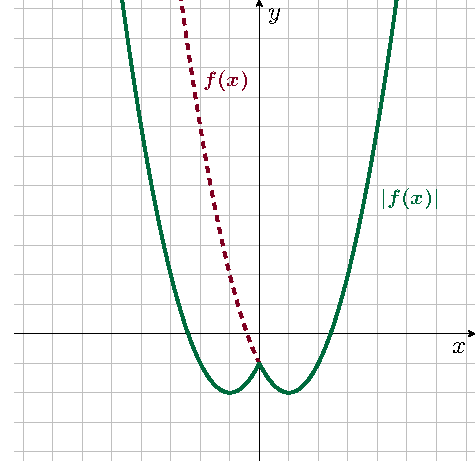
\includegraphics[align=t, width=0.5\textwidth]{../graphs/graph_19/graph_19}
		\end{center}
	\end{minipage}
\end{enumerate}
\end{document}